\section{Methods}
\label{pk:sec:methods}

In this section, we first show how the Bradley--Terry model of pairwise comparisons (the modern name of Zermelo's model), can be expressed in the Gaussian-process framework.
The Gaussian-process viewpoint shifts the focus from \emph{items} (or, in our case, contestants) to \emph{games}: the statistical relationship between outcomes of several games is given by a covariance function.
Second, we present the \emph{player kernel}, a covariance function that relates football matches through lineups.


\subsection{Gaussian-Process Classification Viewpoint}

Suppose that we observe outcomes of comparisons between two items (e.g., two players or two teams) in a universe of items denoted $1, \ldots, N$.
We begin by restricting ourselves to binary outcomes, i.e., we assume that one of the two items necessarily wins.
The Bradley-Terry model postulates that each item $i$ can be represented by a parameter $\theta_i \in \mathbf{R}$, indicative of its relative strength against an opponent.
Given these parameters, the probability of observing the outcome $i \succ j$ is given by
\begin{align}
\label{pk:eq:logistic}
\Prob{i \succ j} = \frac{1}{1 + \exp[-(\theta_i - \theta_j)]} = \frac{1}{1 + \exp(- \bm{\theta}^\Tr \bm{x})},
\end{align}
where $\bm{\theta} = [\theta_i]$ and $\bm{x} \in \mathbf{R}^N$ is such that $x_i = 1$, $x_j = -1$ and $x_k = 0$ for $k \ne i, j$.
As such, the pairwise comparison model can be seen as a special case of logistic regression \citep[Chapter 4]{bishop2006pattern}, where the feature vector simply indicates the winning and losing items.
Furthermore, logistic regression is itself a special case of Gaussian-process classification \cite[Chapter 3]{rasmussen2006gaussian}.

\begin{definition}[Gaussian process]
A \emph{Gaussian process}
\begin{align*}
f(\bm{x}) \sim \mathrm{GP}[m(\bm{x}), k(\bm{x}, \bm{x}')]
\end{align*}
is a stochastic process defined by a mean function $m(\bm{x}) \doteq \Exp{f(\bm{x})}$ and a positive semi-definite covariance (or kernel) function $k(\bm{x}, \bm{x}') \doteq \Cov{f(\bm{x})}{f(\bm{x}')}$.
Given any finite collection of points $\bm{x}_1, \ldots, \bm{x}_M$, the Gaussian process sampled at these points has a multivariate Gaussian distribution
\begin{align*}
\begin{bmatrix}
f(\bm{x}_1) & \cdots & f(\bm{x}_M)
\end{bmatrix} \sim \DNorm{\bm{m}, \bm{K}},
\end{align*}
where $m_u = m(\bm{x}_u)$ and $k_{uv} = k(\bm{x}_u, \bm{x}_v)$.
\end{definition}

It is not hard to show that if $\bm{\theta} \sim \DNorm{\bm{0}, \sigma^2 \bm{I}}$, then $f(\bm{x}) = \bm{\theta}^\Tr \bm{x}$ is a Gaussian process with $m(\bm{x}) = 0$ and $k(\bm{x}, \bm{x}') = \sigma^2 \bm{x}^\top \bm{x}'$.
This enables us to interpret \eqref{pk:eq:logistic} as the likelihood of a Gaussian-process classification model with the logit link function.

The Gaussian-process viewpoint shifts the focus from the parametric representation of the function $f(\bm{x})$ (in the case of \eqref{pk:eq:logistic}, a linear function of items strengths) to the covariance between two function evaluations, as defined by the kernel function $k(\bm{x}, \bm{x}')$.
Intuitively (and informally), the model can simply be specified by stating how similar any two match outcomes are expected to be.
Furthermore, the Gaussian-process viewpoint also makes it possible to take advantage of the vast amount of literature and software related to accurate, efficient, and scalable inference.


\paragraph{Handling Draws}
\citet{rao1967ties} propose an extension of the pairwise comparison model for ternary (win, draw, loss) outcomes.
In this extension, the two different types of outcomes have probabilities
\begin{align*}
\Prob{i \succ j}  &= \frac{1}{1 + \exp[f(\bm{x}) - \alpha]} \\
\Prob{i \equiv j} &= (e^{2 \alpha} - 1) \Prob{i \succ j} \Prob{j \succ i},
\end{align*}
where $\alpha > 0$ is an additional hyperparameter controlling the frequency of draws (see also Section~\ref{fi:sec:ties}).
Because a draw can be written as the product of a win and a loss, model inference can still be performed using only a \emph{binary} Gaussian-process classification model, with the changes needed to the link function being minimal.


\subsection{The Player Kernel}

We now consider an application to football and propose a method to quantify how similar two match outcomes are expected to be.
Let $1, \dots, P$ denote all distinct players appearing in a dataset of matches.
We define a team's \emph{lineup} as the set consisting of the \num{11} players starting the match.
For a given match, let $\mathcal{W}$ and $\mathcal{L}$ be the lineups of the winning and losing teams, respectively.
Define $\bm{z} \in \mathbf{R}^P$ such that $z_p = 1$ if $p \in \mathcal{W}$, $z_p = -1$ if $p \in \mathcal{L}$ and $z_p = 0$ otherwise.
We then define the player kernel as
\begin{align*}
k(\bm{z}, \bm{z}') = \sigma^2 \bm{z}^\top \bm{z}'.
\end{align*}
Intuitively, the function is positive if the same players are lined up in both matches, and the same players win (respectively, lose).
The function is negative when players win one match, but lose the other.
Finally, the function is zero, e.g., when the lineups are completely disjoint.

This kernel implicitly projects every match into the space of players, and defines a notion of similarity in this space.
In the case of national teams qualified to Euro final tournaments, we find that this approach is very useful: a significant part of national teams' players take part in one of the main European leagues and play with or against each other.
International club competitions (such as the UEFA Champions League) further contribute to the ``connectivity'' among players.
Figure~\ref{pk:fig:kernel} illustrates the similarity of matches across different competitions in 2011--2012.


\begin{figure}
  \centering
  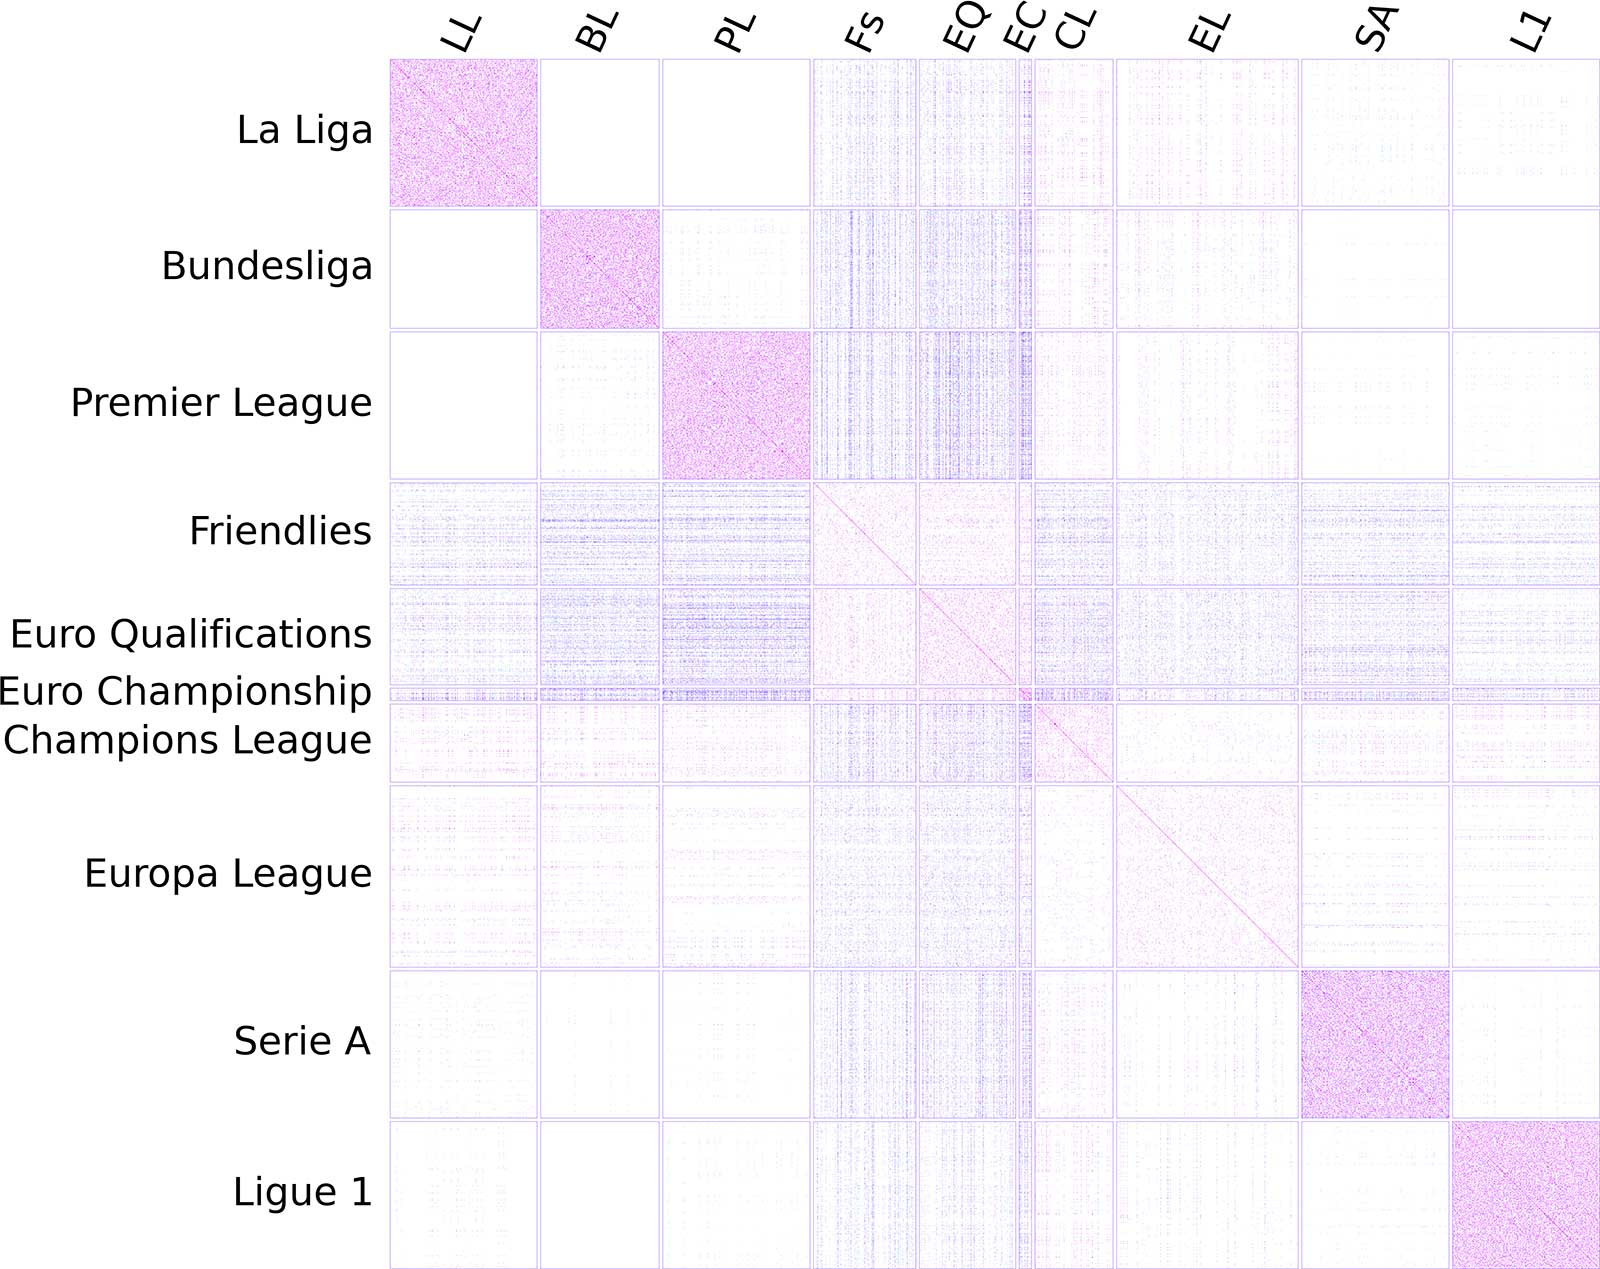
\includegraphics{pk-kernelmatrix}
  \caption{Heat map of the magnitude of the kernel matrix for \num{3184} matches played over the year preceding Euro 2012.
White indicates zero correlation, black indicates non-zero correlation.
Matches between national teams exhibit non-zero covariance with matches of all other competitions.
}
  \label{pk:fig:kernel}
\end{figure}

It is interesting to note that the player kernel corresponds to a linear model over the players.
That is, it is equivalent to assuming that there is one independent skill parameter per player, and that the strength of a team is the sum of its players' skills.
Such a model contains a massive number of parameters (possibly much more than the number of observations), and there is little hope for a reliable estimation of every parameter.
In fact, in Section~\ref{pk:sec:evaluation} we observe that the model is ``weakly'' parametric: the number of distinct players usually grows with the number of matches observed.
The kernel-based viewpoint that we take emphasizes the fact that estimating these parameters explicitly is \emph{not} necessary.

\paragraph{Relation to TrueSkill}
Our Gaussian-process model coupled with the player kernel is very similar to TrueSkill \citep{herbrich2006trueskill}.
The most important difference is that we take advantage of the dual representation and operate in the space of matches, instead of in the space of players.
Beyond the conceptual reasons outlined above, the model makes inference less computationally intensive for the datasets that we consider.
